%
% volint.tex
%
% (c) 2025 Prof Dr Andreas Müller, OST Ostschweizer Fachhochschule
%
\documentclass[tikz]{standalone}
\usepackage{times}
\usepackage{amsmath}
\usepackage{txfonts}
\usepackage[utf8]{inputenc}
\usepackage{graphics}
\usetikzlibrary{arrows,intersections,math}
\usepackage{ifthen}
\begin{document}

\newboolean{showgrid}
\setboolean{showgrid}{false}
\def\breite{7}
\def\hoehe{7}

\definecolor{gruen}{rgb}{0,0.6,0.2}

\begin{tikzpicture}[>=latex,thick]

\clip (-6.3,-7.5) rectangle (6.3,7.3);

% Povray Bild
\begin{scope}[yshift=3.7cm]
	\node at (0,0) {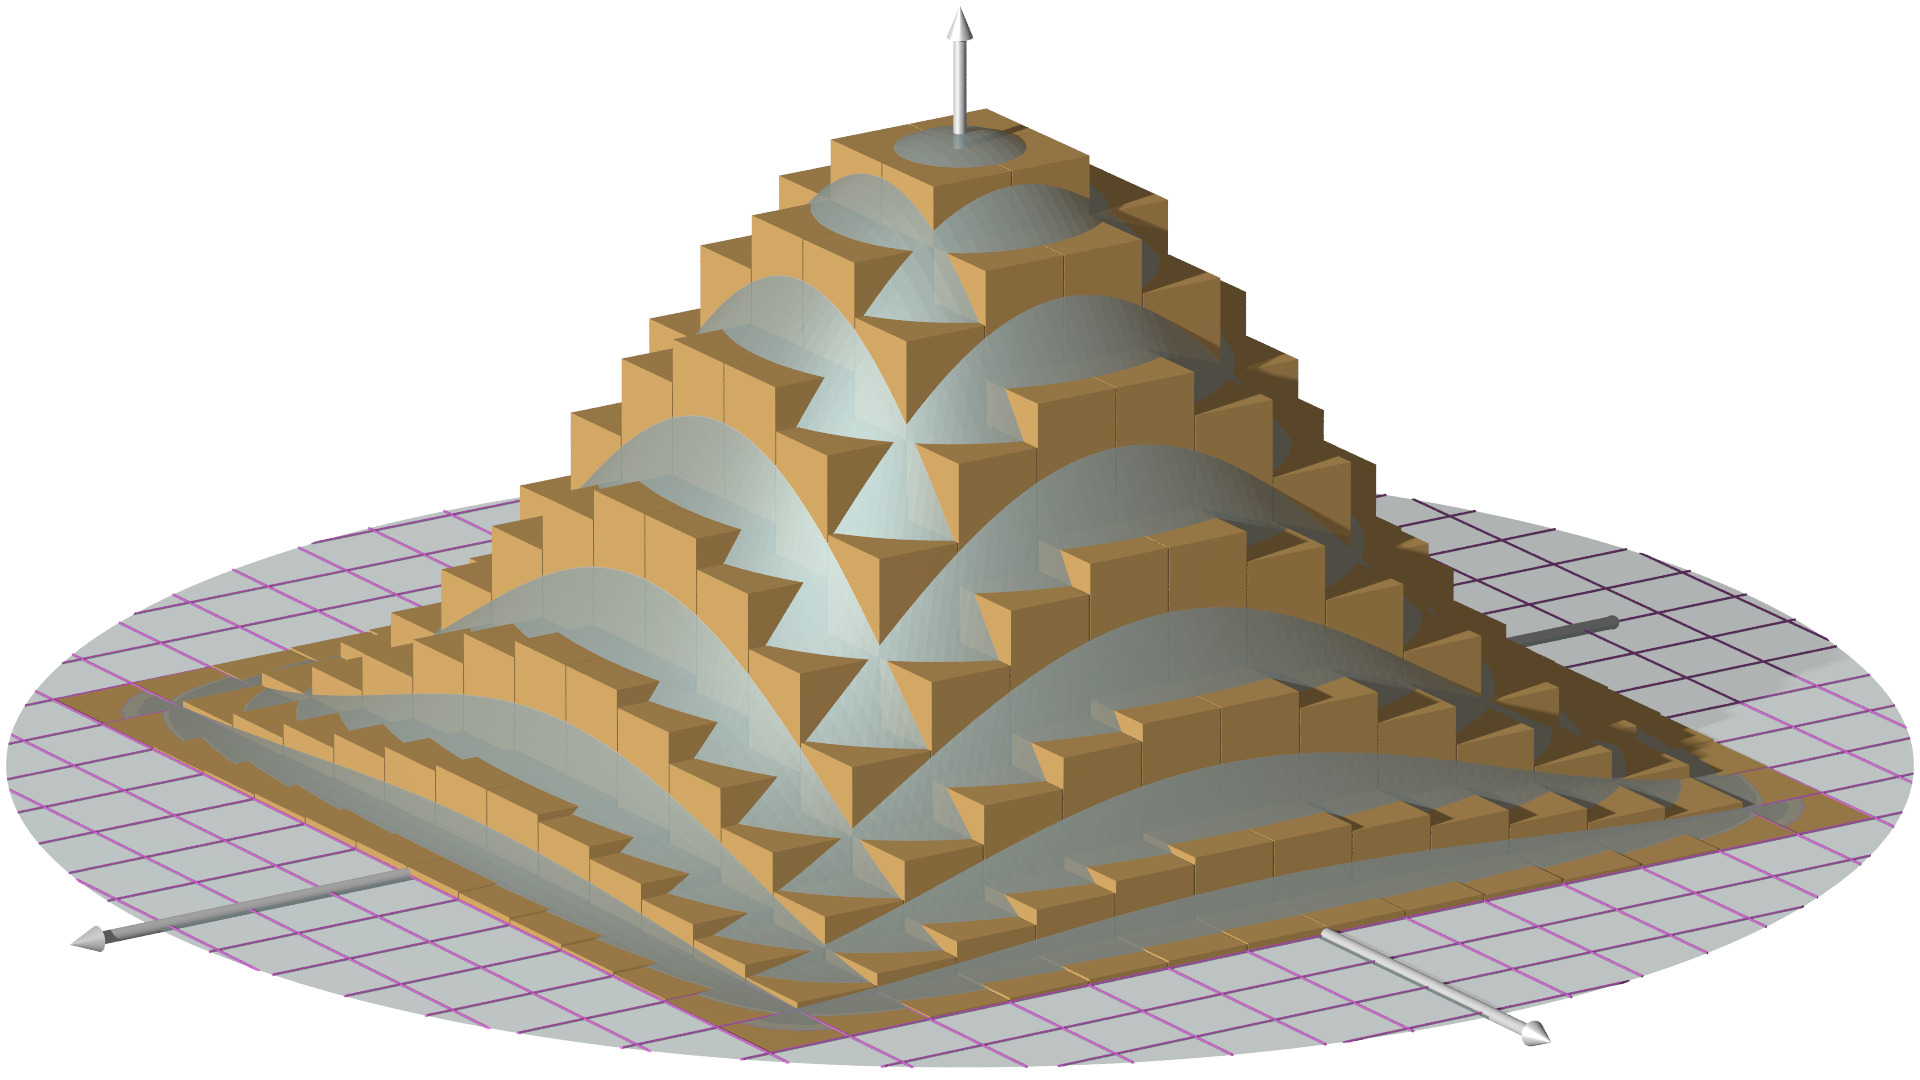
\includegraphics[width=12.6cm]{volintx.jpg}};
	\node at (-6.0,-2.6) {$x^1$};
	\node at (4.1,-3.2) {$x^2$};
	\node at (0.3,3.4) {$z$};
\end{scope}

\begin{scope}[yshift=-3.7cm]
	\node at (0,0) {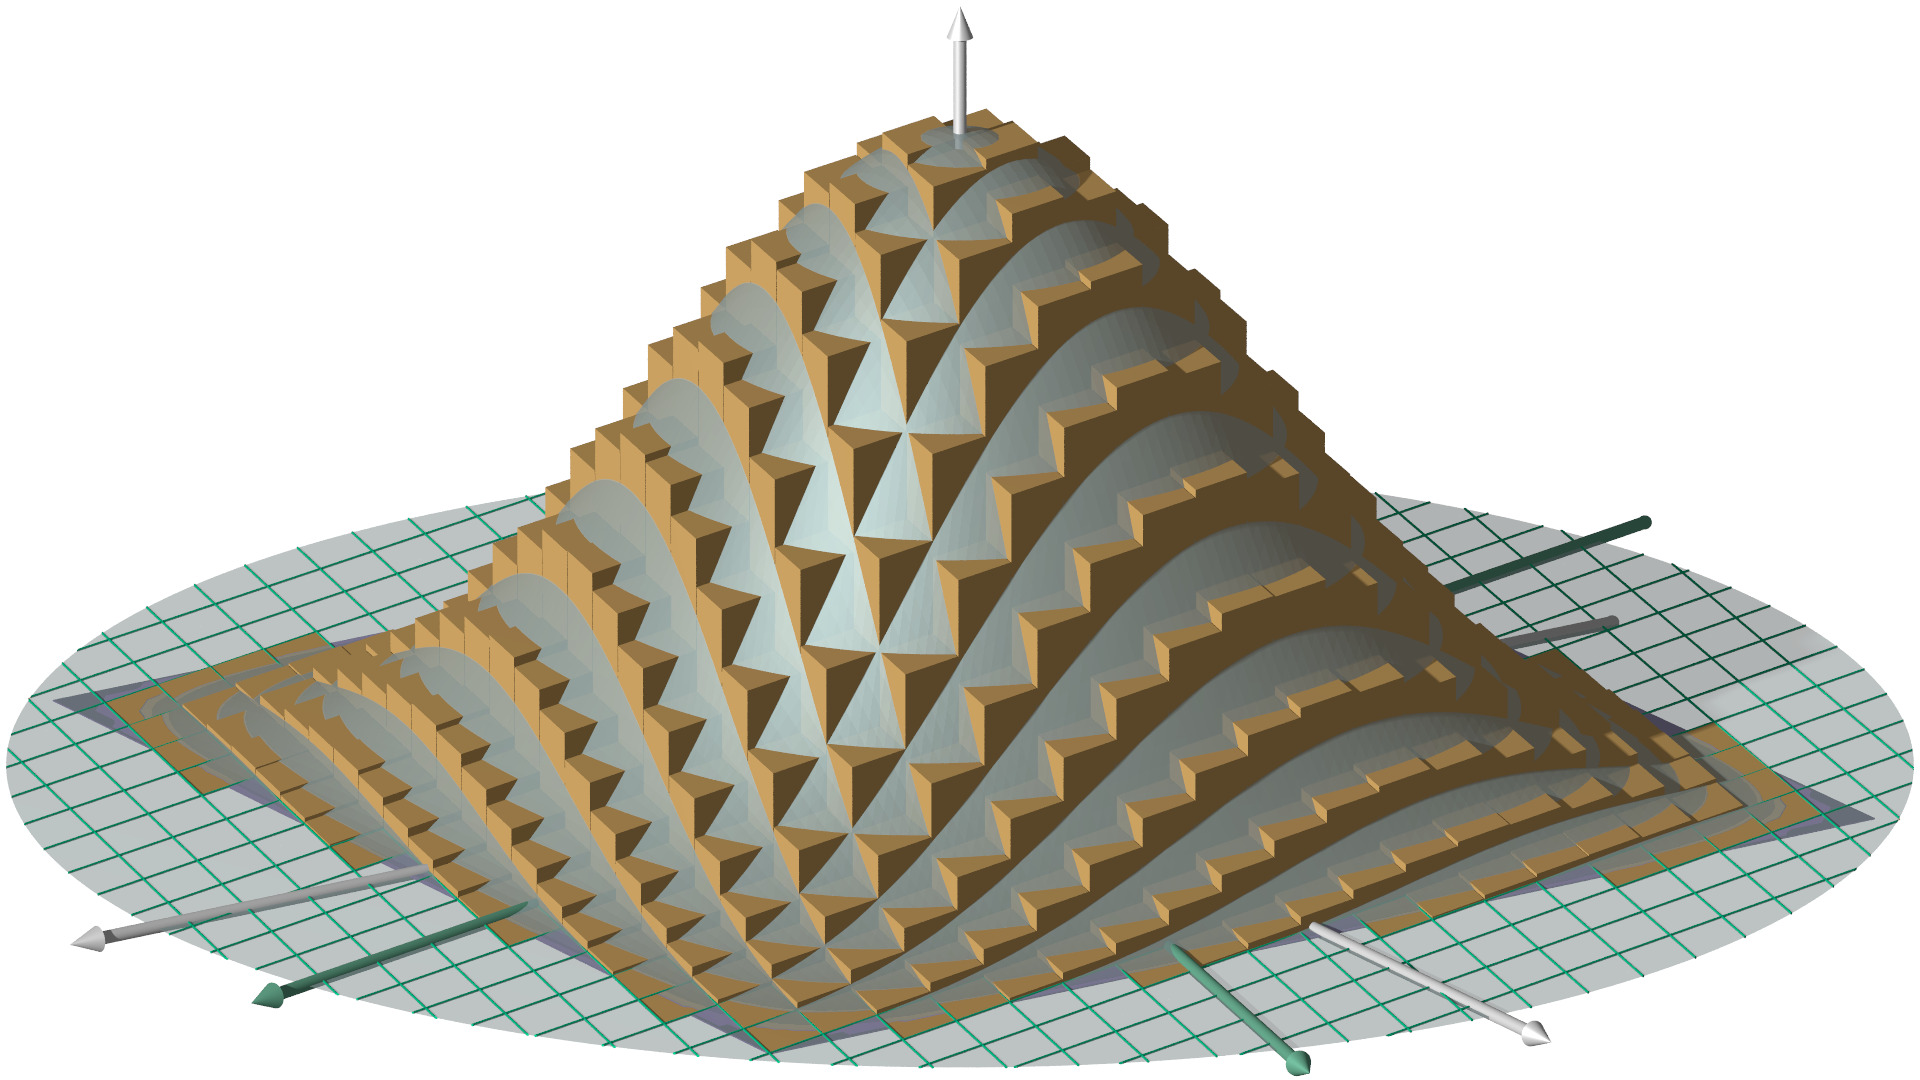
\includegraphics[width=12.6cm]{volinty.jpg}};
	\node at (-6.0,-2.6) {$x^1$};
	\node at (4.1,-3.2) {$x^2$};
	\node at (0.3,3.4) {$z$};
	\node[color=gruen] at (-4.80,-3.15) {$y^1$};
	\node[color=gruen] at (2.55,-3.55) {$y^2$};
\end{scope}

% Gitter
\ifthenelse{\boolean{showgrid}}{
\draw[step=0.1,line width=0.1pt] (-\breite,-\hoehe) grid (\breite, \hoehe);
\draw[step=0.5,line width=0.4pt] (-\breite,-\hoehe) grid (\breite, \hoehe);
\draw                            (-\breite,-\hoehe) grid (\breite, \hoehe);
\fill (0,0) circle[radius=0.05];
}{}

\end{tikzpicture}

\end{document}

